% Options for packages loaded elsewhere
\PassOptionsToPackage{unicode}{hyperref}
\PassOptionsToPackage{hyphens}{url}
\PassOptionsToPackage{dvipsnames,svgnames*,x11names*}{xcolor}
%
\documentclass[
  10pt,
]{article}
\usepackage{lmodern}
\usepackage{setspace}
\usepackage{amssymb,amsmath}
\usepackage{ifxetex,ifluatex}
\ifnum 0\ifxetex 1\fi\ifluatex 1\fi=0 % if pdftex
  \usepackage[T1]{fontenc}
  \usepackage[utf8]{inputenc}
  \usepackage{textcomp} % provide euro and other symbols
\else % if luatex or xetex
  \usepackage{unicode-math}
  \defaultfontfeatures{Scale=MatchLowercase}
  \defaultfontfeatures[\rmfamily]{Ligatures=TeX,Scale=1}
  \setmainfont[]{DejaVu Serif}
  \setmonofont[]{DejaVu Sans Mono}
\fi
% Use upquote if available, for straight quotes in verbatim environments
\IfFileExists{upquote.sty}{\usepackage{upquote}}{}
\IfFileExists{microtype.sty}{% use microtype if available
  \usepackage[]{microtype}
  \UseMicrotypeSet[protrusion]{basicmath} % disable protrusion for tt fonts
}{}
\makeatletter
\@ifundefined{KOMAClassName}{% if non-KOMA class
  \IfFileExists{parskip.sty}{%
    \usepackage{parskip}
  }{% else
    \setlength{\parindent}{0pt}
    \setlength{\parskip}{6pt plus 2pt minus 1pt}}
}{% if KOMA class
  \KOMAoptions{parskip=half}}
\makeatother
\usepackage{xcolor}
\IfFileExists{xurl.sty}{\usepackage{xurl}}{} % add URL line breaks if available
\IfFileExists{bookmark.sty}{\usepackage{bookmark}}{\usepackage{hyperref}}
\hypersetup{
  colorlinks=true,
  linkcolor=red,
  filecolor=red,
  citecolor=red,
  urlcolor=red,
  pdfcreator={LaTeX via pandoc}}
\urlstyle{same} % disable monospaced font for URLs
\usepackage[margin=0.3cm,top=0.5cm,bottom=0.5cm,left=0.3cm,right=0.3cm,includeheadfoot]{geometry}
\usepackage{color}
\usepackage{fancyvrb}
\newcommand{\VerbBar}{|}
\newcommand{\VERB}{\Verb[commandchars=\\\{\}]}
\DefineVerbatimEnvironment{Highlighting}{Verbatim}{commandchars=\\\{\}}
% Add ',fontsize=\small' for more characters per line
\newenvironment{Shaded}{}{}
\newcommand{\AlertTok}[1]{\textcolor[rgb]{1.00,0.00,0.00}{\textbf{#1}}}
\newcommand{\AnnotationTok}[1]{\textcolor[rgb]{0.38,0.63,0.69}{\textbf{\textit{#1}}}}
\newcommand{\AttributeTok}[1]{\textcolor[rgb]{0.49,0.56,0.16}{#1}}
\newcommand{\BaseNTok}[1]{\textcolor[rgb]{0.25,0.63,0.44}{#1}}
\newcommand{\BuiltInTok}[1]{#1}
\newcommand{\CharTok}[1]{\textcolor[rgb]{0.25,0.44,0.63}{#1}}
\newcommand{\CommentTok}[1]{\textcolor[rgb]{0.38,0.63,0.69}{\textit{#1}}}
\newcommand{\CommentVarTok}[1]{\textcolor[rgb]{0.38,0.63,0.69}{\textbf{\textit{#1}}}}
\newcommand{\ConstantTok}[1]{\textcolor[rgb]{0.53,0.00,0.00}{#1}}
\newcommand{\ControlFlowTok}[1]{\textcolor[rgb]{0.00,0.44,0.13}{\textbf{#1}}}
\newcommand{\DataTypeTok}[1]{\textcolor[rgb]{0.56,0.13,0.00}{#1}}
\newcommand{\DecValTok}[1]{\textcolor[rgb]{0.25,0.63,0.44}{#1}}
\newcommand{\DocumentationTok}[1]{\textcolor[rgb]{0.73,0.13,0.13}{\textit{#1}}}
\newcommand{\ErrorTok}[1]{\textcolor[rgb]{1.00,0.00,0.00}{\textbf{#1}}}
\newcommand{\ExtensionTok}[1]{#1}
\newcommand{\FloatTok}[1]{\textcolor[rgb]{0.25,0.63,0.44}{#1}}
\newcommand{\FunctionTok}[1]{\textcolor[rgb]{0.02,0.16,0.49}{#1}}
\newcommand{\ImportTok}[1]{#1}
\newcommand{\InformationTok}[1]{\textcolor[rgb]{0.38,0.63,0.69}{\textbf{\textit{#1}}}}
\newcommand{\KeywordTok}[1]{\textcolor[rgb]{0.00,0.44,0.13}{\textbf{#1}}}
\newcommand{\NormalTok}[1]{#1}
\newcommand{\OperatorTok}[1]{\textcolor[rgb]{0.40,0.40,0.40}{#1}}
\newcommand{\OtherTok}[1]{\textcolor[rgb]{0.00,0.44,0.13}{#1}}
\newcommand{\PreprocessorTok}[1]{\textcolor[rgb]{0.74,0.48,0.00}{#1}}
\newcommand{\RegionMarkerTok}[1]{#1}
\newcommand{\SpecialCharTok}[1]{\textcolor[rgb]{0.25,0.44,0.63}{#1}}
\newcommand{\SpecialStringTok}[1]{\textcolor[rgb]{0.73,0.40,0.53}{#1}}
\newcommand{\StringTok}[1]{\textcolor[rgb]{0.25,0.44,0.63}{#1}}
\newcommand{\VariableTok}[1]{\textcolor[rgb]{0.10,0.09,0.49}{#1}}
\newcommand{\VerbatimStringTok}[1]{\textcolor[rgb]{0.25,0.44,0.63}{#1}}
\newcommand{\WarningTok}[1]{\textcolor[rgb]{0.38,0.63,0.69}{\textbf{\textit{#1}}}}
\setlength{\emergencystretch}{3em} % prevent overfull lines
\providecommand{\tightlist}{%
  \setlength{\itemsep}{0pt}\setlength{\parskip}{0pt}}
\setcounter{secnumdepth}{3}
% Enable graphics inclusion and ensure figure numbering works
\usepackage{graphicx}
\renewcommand{\figurename}{Figure}

% Configure fonts for Unicode support with fallbacks
\usepackage{newunicodechar}
\newunicodechar{⁴}{\textsuperscript{4}}
\newunicodechar{₄}{\textsubscript{4}}

% Configure hyperref colors consistently
\AtBeginDocument{
% Override pandoc's hidelinks setting with consistent options
\hypersetup{
    colorlinks=true,
    allcolors=red,
    linkcolor=red,
    urlcolor=red,
    citecolor=red,
    filecolor=red,
    menucolor=red,
    linktoc=all
}
}

\title{Optimization in 4D}
\author{Daniel Ari Friedman\\ ORCID: 0000-0001-6232-9096\\ Email: daniel@activeinference.institute}
\date{August 14, 2025}

\begin{document}
\maketitle

{
\hypersetup{linkcolor=red}
\setcounter{tocdepth}{3}
\tableofcontents
}
\setstretch{1.0}
\hypertarget{optimization-in-4d-namespaces-and-quadray-lattice-methods}{%
\section{Optimization in 4D (Namespaces and Quadray-Lattice
Methods)}\label{optimization-in-4d-namespaces-and-quadray-lattice-methods}}

Here we review the optimization methods used in this manuscript. We
review the Nelder--Mead method, which is a simple and robust
optimization method that is well-suited to the Quadray 4D lattice. We
also review the discrete IVM descent method, which is a more
sophisticated optimization method that is well-suited to the Quadray
lattice as well.

\hypertarget{quadray-adaptive-neldermead-fuller.4d}{%
\subsection{Quadray-Adaptive Nelder--Mead
(Fuller.4D)}\label{quadray-adaptive-neldermead-fuller.4d}}

\begin{itemize}
\tightlist
\item
  Initialization: choose 4 integer quadray vertices forming a
  non-degenerate simplex (e.g., basis + one mixed point such as
  (1,1,1,0)).
\item
  Reflection/Expansion/Contraction: compute candidate; round to nearest
  integer; renormalize by adding/subtracting (k,k,k,k) to enforce
  non-negativity and at least one zero.
\item
  Shrink: discrete contraction of all vertices toward the best vertex
  along tetrahedral axes.
\end{itemize}

Standard Nelder--Mead coefficients (typical choices):

\begin{itemize}
\tightlist
\item
  \textbf{Reflection} \(\alpha = 1\)
\item
  \textbf{Expansion} \(\gamma \approx 2\)
\item
  \textbf{Contraction} \(\rho \approx 0.5\)
\item
  \textbf{Shrink} \(\sigma \approx 0.5\)
\end{itemize}

References: original Nelder--Mead method and common parameterizations in
optimization texts and survey articles; see overview:
\href{https://en.wikipedia.org/wiki/Nelder\%E2\%80\%93Mead_method}{Nelder--Mead
method}.

\hypertarget{volume-level-dynamics}{%
\subsection{Volume-Level Dynamics}\label{volume-level-dynamics}}

\begin{itemize}
\tightlist
\item
  Simplex volume decreases in discrete integer steps, creating stable
  plateaus (``energy levels'').
\item
  Termination: when volume stabilizes at a minimal level and function
  spread is below tolerance.
\item
  Monitoring: track integer simplex volume and the objective spread at
  each iteration for convergence diagnostics.
\end{itemize}

\hypertarget{pseudocode-sketch}{%
\subsection{Pseudocode (Sketch)}\label{pseudocode-sketch}}

\begin{verbatim}
while not converged:
  order vertices by objective
  centroid of best three
  propose reflected (then possibly expanded/contracted) point
  project to integer quadray; renormalize with (k,k,k,k)
  accept per standard tests; else shrink toward best
  update integer volume and function spread trackers
\end{verbatim}

\hypertarget{figures}{%
\subsubsection{Figures}\label{figures}}

\begin{figure}[htbp]
\centering
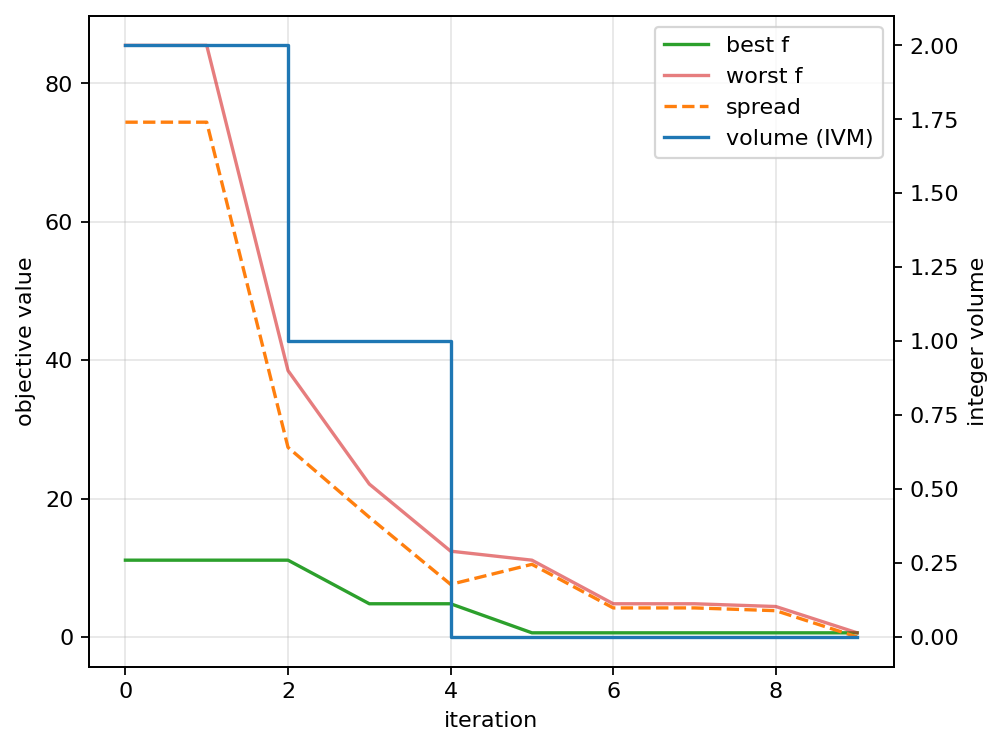
\includegraphics[width=0.9\textwidth]{figures/simplex_trace.png}
\caption{Optimization trace for discrete Nelder–Mead in the Quadray lattice. Best/worst objective values and spread (left axis) with integer tetra-volume (right axis) per iteration. See the MP4 for the full simplex trajectory.}
\label{fig:simplex_trace}
\end{figure}

\begin{figure}[htbp]
\centering
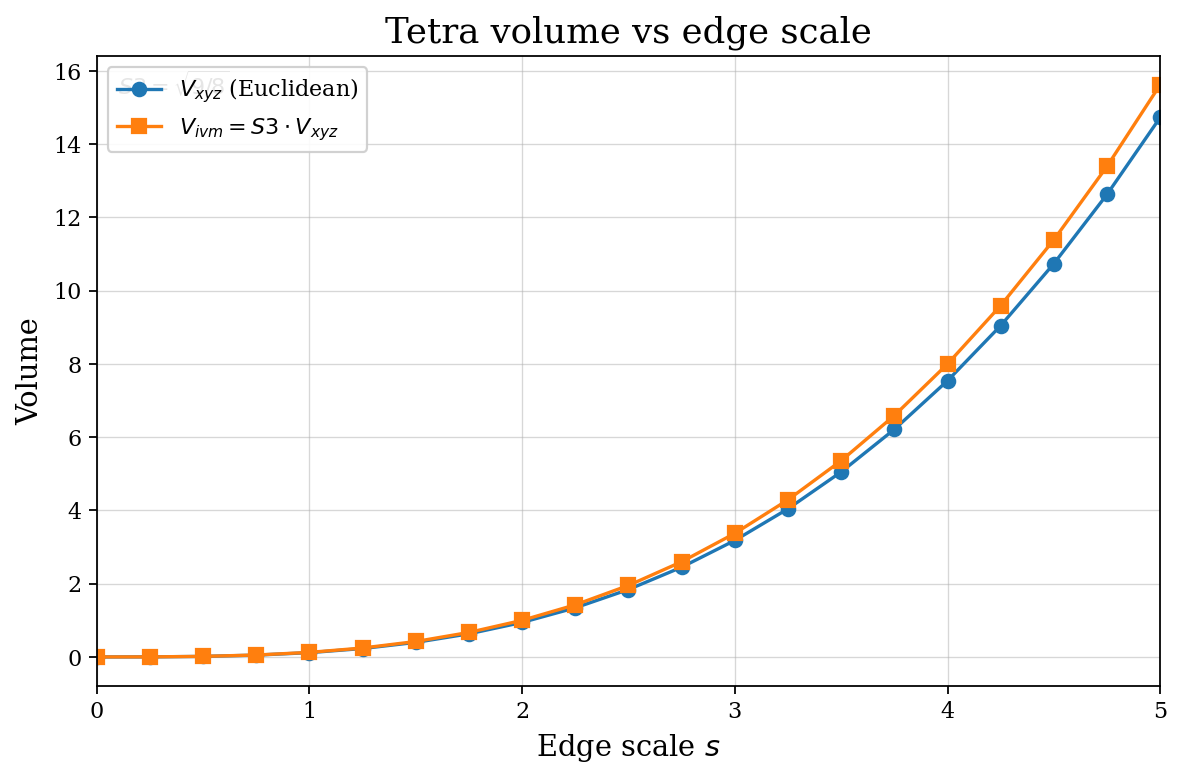
\includegraphics[width=0.9\textwidth]{figures/volumes_scale_plot.png}
\caption{Tetra volume vs edge scale. Two curves: Euclidean volume $V_{xyz}$ and IVM-converted $V_{ivm}=S3\cdot V_{xyz}$; axes labeled; $S3$ annotated; data saved as CSV/NPZ.}
\label{fig:volumes_scale}
\end{figure}

As shown in Figure \ref{fig:simplex_final}, the discrete Nelder--Mead
converges on plateaus; Figure \ref{fig:volumes_scale} summarizes the
scaling behavior used in volume diagnostics.

\begin{figure}[htbp]
\centering
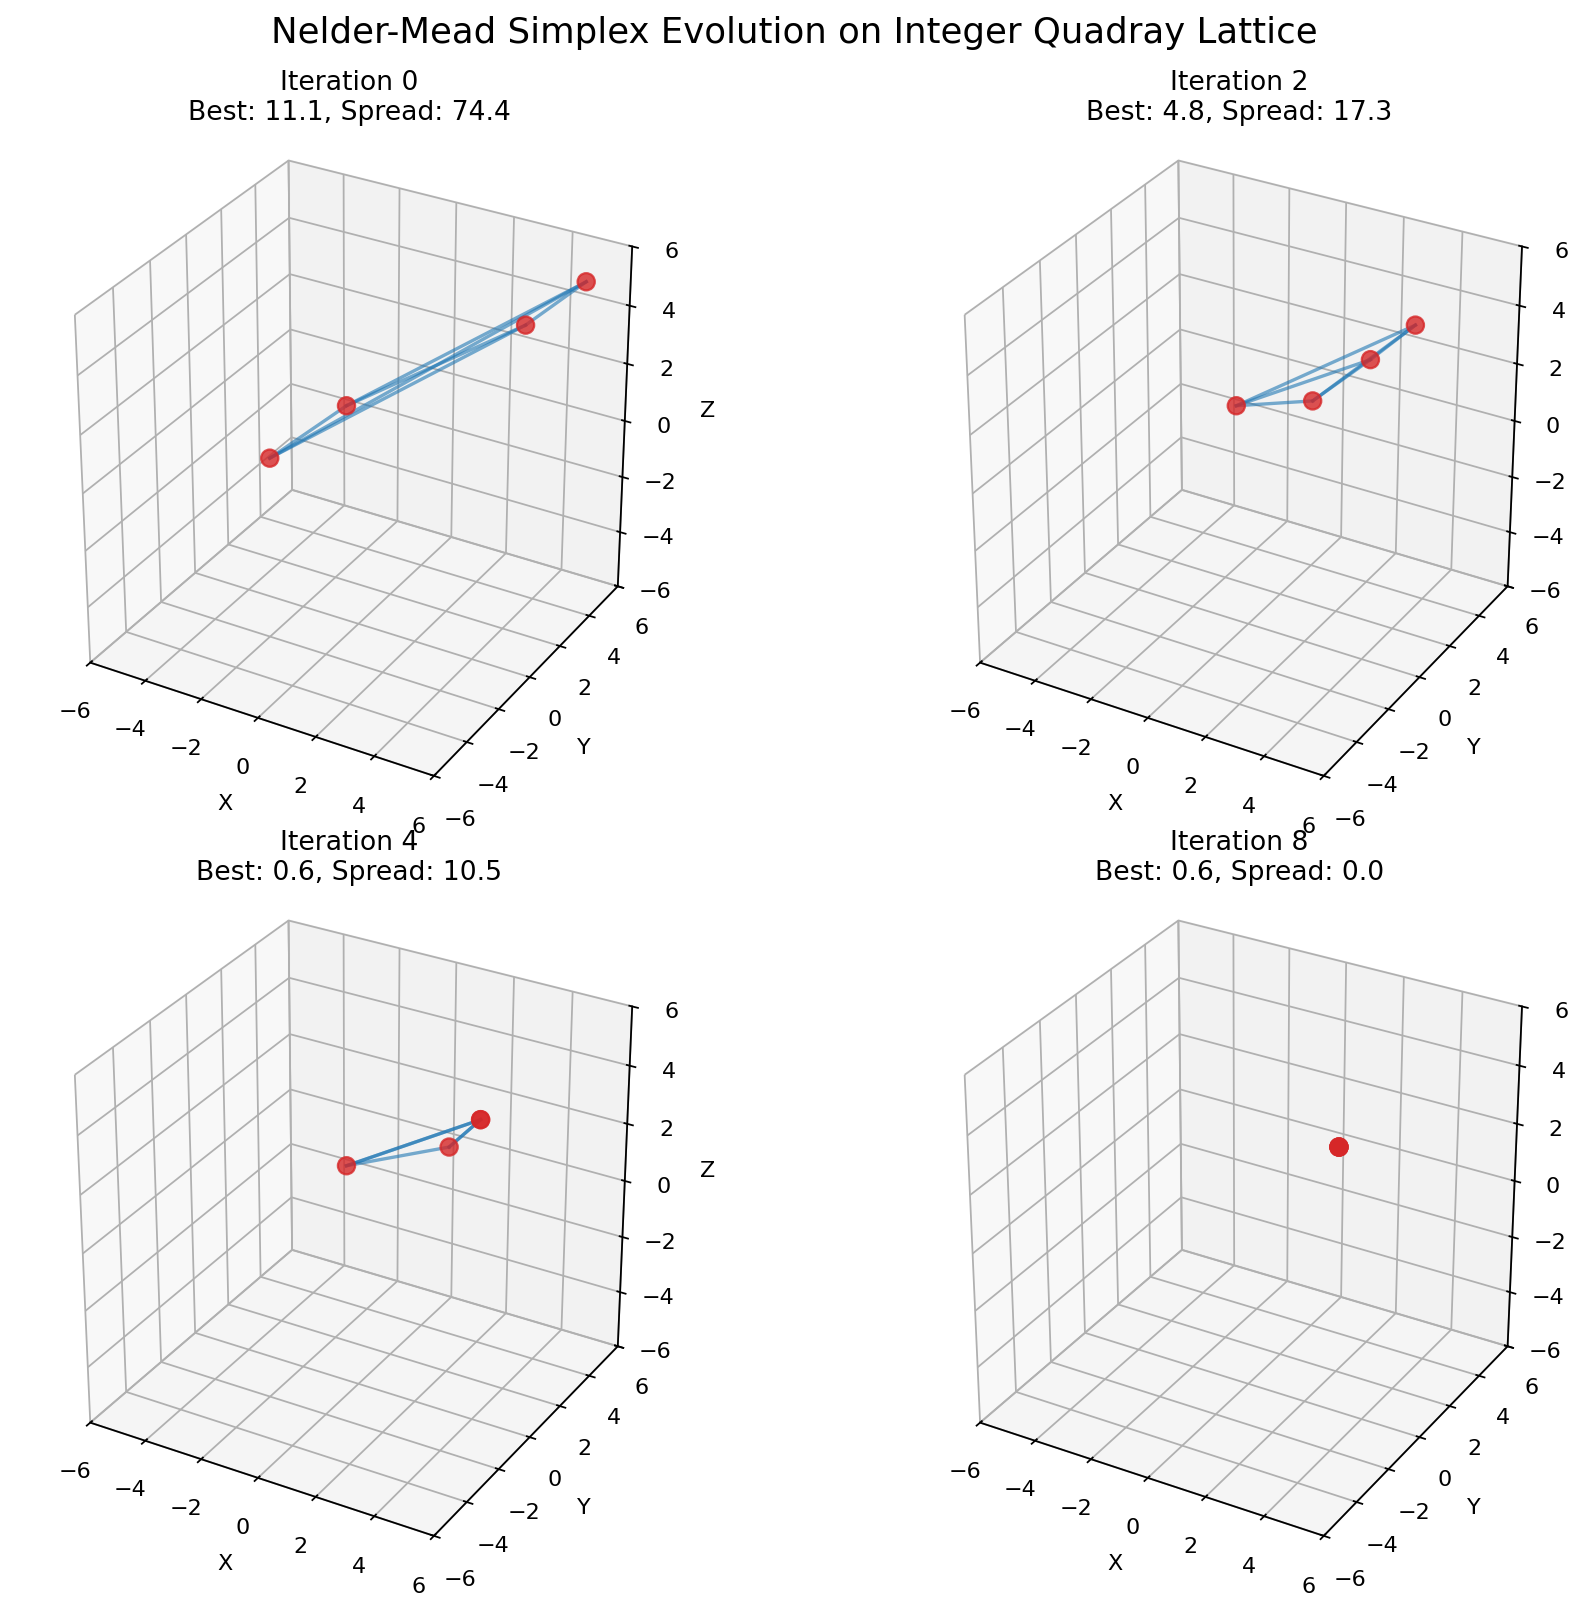
\includegraphics[width=0.9\textwidth]{figures/simplex_final.png}
\caption{Final converged simplex configuration.}
\label{fig:simplex_final}
\end{figure}

Raw artifacts: the full trajectory animation
\texttt{simplex\_animation.mp4} and per-frame vertices
(\texttt{simplex\_animation\_vertices.csv}/\texttt{.npz}) are available
in \texttt{quadmath/output/}. The full optimization trajectory is
provided as an animation (MP4) in the repository's output directory.

\hypertarget{discrete-lattice-descent-information-theoretic-variant}{%
\subsection{Discrete Lattice Descent (Information-Theoretic
Variant)}\label{discrete-lattice-descent-information-theoretic-variant}}

\begin{itemize}
\tightlist
\item
  Integer-valued descent over the IVM using the 12 neighbor moves
  (permutations of \{2,1,1,0\}), snapping to the canonical
  representative via projective normalization.
\item
  Objective can be geometric (e.g., Euclidean in an embedding) or
  information-theoretic (e.g., local free-energy proxy); monotone
  decrease is guaranteed by greedy selection.
\item
  API: \texttt{discrete\_ivm\_descent} in
  \texttt{src/discrete\_variational.py}. Animation helper:
  \texttt{animate\_discrete\_path} in \texttt{src/visualize.py}.
\end{itemize}

Short snippet (paper reproducibility):

\begin{Shaded}
\begin{Highlighting}[]
\ImportTok{from}\NormalTok{ quadray }\ImportTok{import}\NormalTok{ Quadray, DEFAULT\_EMBEDDING, to\_xyz}
\ImportTok{from}\NormalTok{ discrete\_variational }\ImportTok{import}\NormalTok{ discrete\_ivm\_descent}
\ImportTok{from}\NormalTok{ visualize }\ImportTok{import}\NormalTok{ animate\_discrete\_path}

\KeywordTok{def}\NormalTok{ f(q: Quadray) }\OperatorTok{{-}\textgreater{}} \BuiltInTok{float}\NormalTok{:}
\NormalTok{    x, y, z }\OperatorTok{=}\NormalTok{ to\_xyz(q, DEFAULT\_EMBEDDING)}
    \ControlFlowTok{return}\NormalTok{ (x }\OperatorTok{{-}} \FloatTok{0.5}\NormalTok{)}\OperatorTok{**}\DecValTok{2} \OperatorTok{+}\NormalTok{ (y }\OperatorTok{+} \FloatTok{0.2}\NormalTok{)}\OperatorTok{**}\DecValTok{2} \OperatorTok{+}\NormalTok{ (z }\OperatorTok{{-}} \FloatTok{0.1}\NormalTok{)}\OperatorTok{**}\DecValTok{2}

\NormalTok{path }\OperatorTok{=}\NormalTok{ discrete\_ivm\_descent(f, Quadray(}\DecValTok{6}\NormalTok{,}\DecValTok{0}\NormalTok{,}\DecValTok{0}\NormalTok{,}\DecValTok{0}\NormalTok{))}
\NormalTok{animate\_discrete\_path(path)}
\end{Highlighting}
\end{Shaded}

\hypertarget{convergence-and-robustness}{%
\subsection{Convergence and
Robustness}\label{convergence-and-robustness}}

\begin{itemize}
\tightlist
\item
  Discrete steps reduce numerical drift; improved stability
  vs.~unconstrained Cartesian.
\item
  Natural regularization from volume quantization; fewer wasted
  evaluations.
\item
  Compatible with Gauss--Newton/Natural Gradient guidance using FIM for
  metric-aware steps (Amari, natural gradient).
\end{itemize}

\hypertarget{information-geometric-view-einstein.4d-analogy-in-metric-form}{%
\subsection{Information-Geometric View (Einstein.4D analogy in metric
form)}\label{information-geometric-view-einstein.4d-analogy-in-metric-form}}

\begin{itemize}
\tightlist
\item
  \textbf{Fisher Information as metric}: use the empirical estimator
  \texttt{F\ =\ (1/N)\ \textbackslash{}sum\ g\ g\^{}\textbackslash{}top}
  from \texttt{fisher\_information\_matrix} to analyze curvature of the
  objective with respect to parameters. See
  \href{https://en.wikipedia.org/wiki/Fisher_information}{Fisher
  information}.
\item
  \textbf{Curvature directions}: leading eigenvalues/eigenvectors of
  \texttt{F} (see \texttt{fim\_eigenspectrum}) reveal stiff and sloppy
  directions; this supports step-size selection and preconditioning.
\item
  \textbf{Figures}: empirical FIM heatmap (Figure
  \ref{fig:fisher_information_matrix}) and eigenspectrum (Figure
  \ref{fig:fim_eigenspectrum}). Raw data available as NPZ/CSV in
  \texttt{quadmath/output/}.
\end{itemize}

\begin{figure}[htbp]
\centering
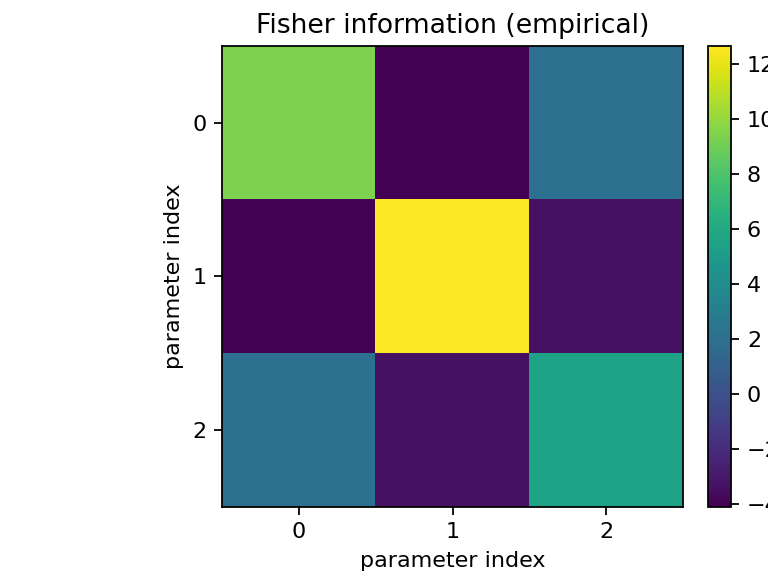
\includegraphics[width=0.9\textwidth]{figures/fisher_information_matrix.png}
\caption{Empirical Fisher information heatmap (entries $F_{ij}$ estimated via outer products of per-sample gradients; model: noisy linear regression; evaluated at misspecified parameters $w_\text{est}$ vs ground truth $w_\text{true}$; colorbar shows curvature scale).}
\label{fig:fisher_information_matrix}
\end{figure}

\begin{figure}[htbp]
\centering
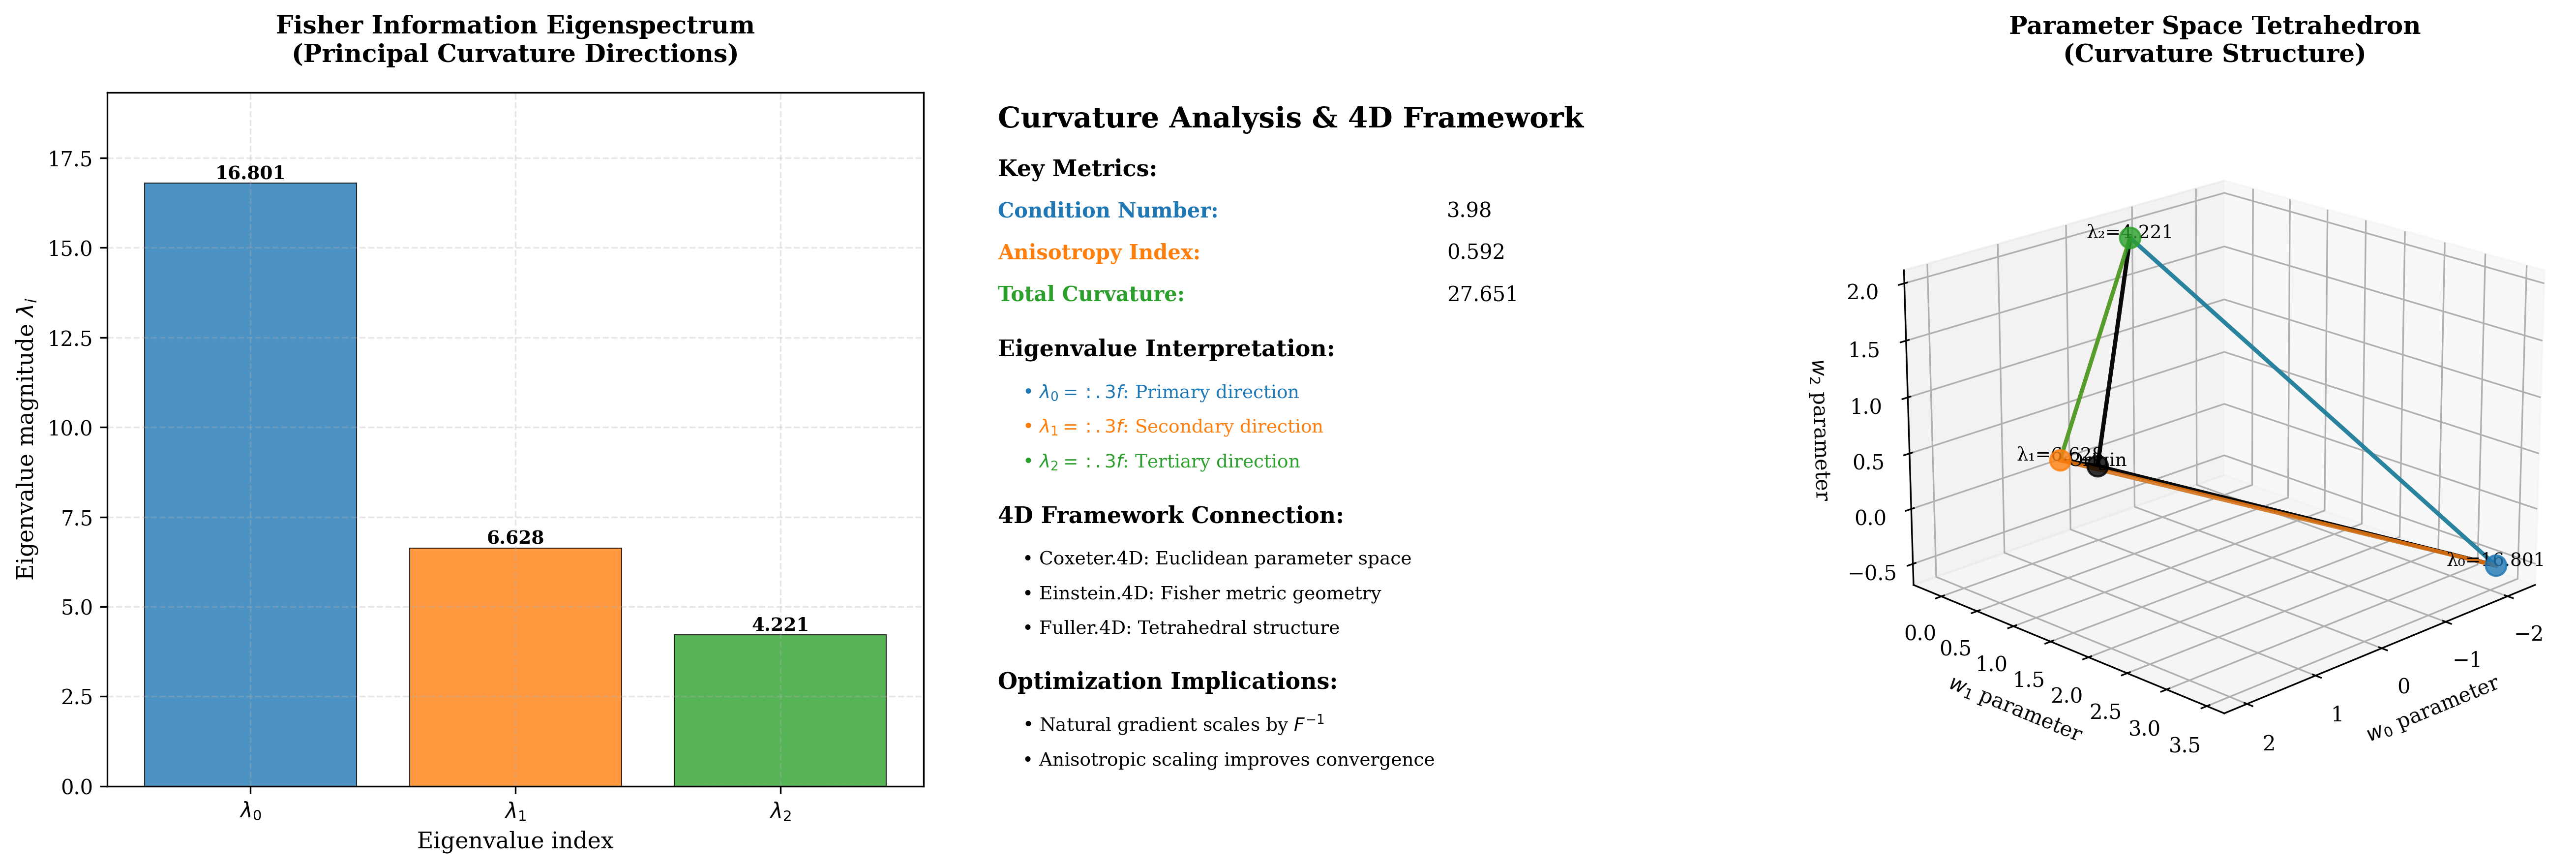
\includegraphics[width=0.9\textwidth]{figures/fisher_information_eigenspectrum.png}
\caption{Fisher information eigenspectrum (principal curvatures along eigenvectors of $F$; eigenvalues $\lambda_i$ sorted descending; highlights stiff vs. sloppy directions).}
\label{fig:fim_eigenspectrum}
\end{figure}

\begin{figure}[htbp]
\centering
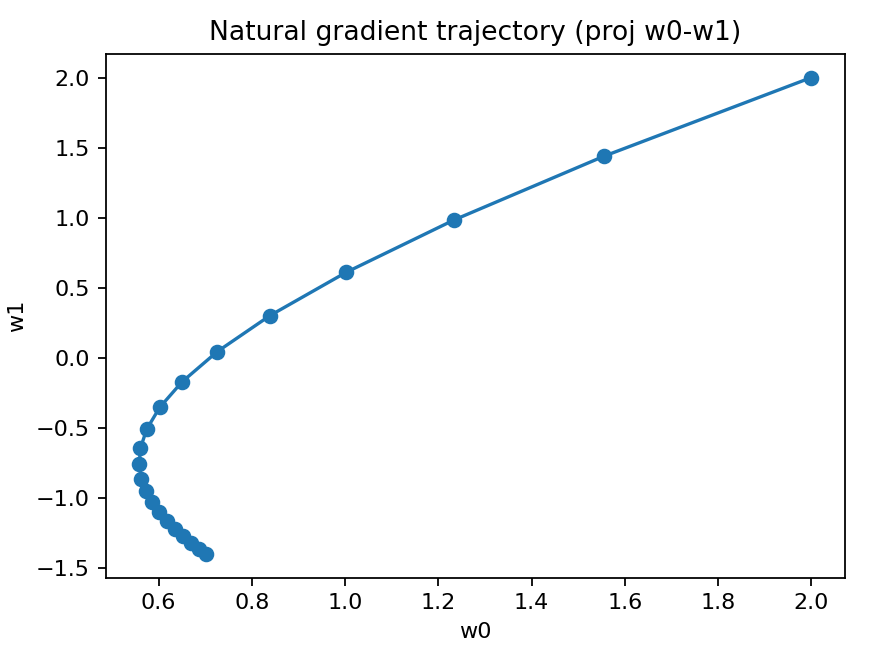
\includegraphics[width=0.9\textwidth]{figures/natural_gradient_path.png}
\caption{Natural gradient trajectory on a quadratic bowl (projection in $w_0$–$w_1$ plane); $A=\begin{bmatrix}3 & 0.5 & 0\\ 0.5 & 2 & 0\\ 0 & 0 & 1\end{bmatrix}$, step size $\eta=0.5$, damped inverse Fisher $F + 10^{-3} I$; raw path in CSV/NPZ.}
\label{fig:natural_gradient_path}
\end{figure}

\begin{figure}[htbp]
\centering
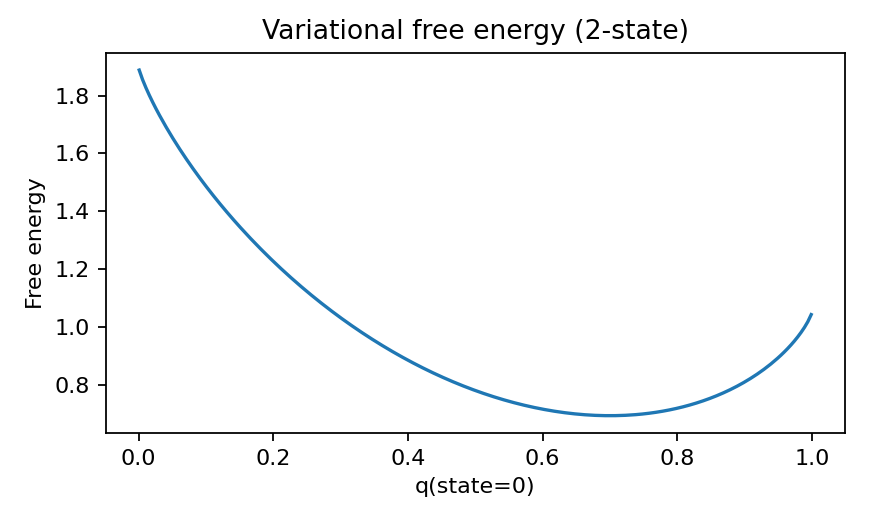
\includegraphics[width=0.9\textwidth]{figures/free_energy_curve.png}
\caption{Free energy curve for a 2-state model.}
\label{fig:free_energy_curve}
\end{figure}

\begin{itemize}
\tightlist
\item
  \textbf{Quadray relevance}: block-structured and symmetric patterns
  often arise under quadray parameterizations, simplifying \texttt{F}
  inversion for natural-gradient steps.
\end{itemize}

\hypertarget{multi-objective-and-higher-dimensional-notes-coxeter.4d-perspective}{%
\subsection{Multi-Objective and Higher-Dimensional Notes (Coxeter.4D
perspective)}\label{multi-objective-and-higher-dimensional-notes-coxeter.4d-perspective}}

\begin{itemize}
\tightlist
\item
  Multi-objective: vertices encode trade-offs; simplex faces approximate
  Pareto surfaces; integer volume measures solution diversity.
\item
  Higher dimensions: decompose higher-dimensional simplexes into
  tetrahedra; sum integer volumes to extend quantization.
\end{itemize}

\hypertarget{dsolutions-optimization-context-and-educational-implementations}{%
\subsection{4dsolutions optimization context and educational
implementations}\label{dsolutions-optimization-context-and-educational-implementations}}

The optimization methods developed here build upon and complement the
extensive computational framework in Kirby Urner's
\href{https://github.com/4dsolutions}{4dsolutions ecosystem}:

\begin{itemize}
\item
  \textbf{Algorithmic foundations}: Our \texttt{nelder\_mead\_quadray}
  and \texttt{discrete\_ivm\_descent} methods extend the vector
  operations and volume calculations implemented in
  \href{https://github.com/4dsolutions/m4w/blob/main/qrays.py}{\texttt{qrays.py}}
  and
  \href{https://github.com/4dsolutions/m4w/blob/main/tetravolume.py}{\texttt{tetravolume.py}}.
\item
  \textbf{Educational precedents}: Interactive optimization
  demonstrations appear in
  \href{https://github.com/4dsolutions/School_of_Tomorrow}{School\_of\_Tomorrow
  notebooks}, particularly volume tracking and CCP navigation in
  \href{https://github.com/4dsolutions/School_of_Tomorrow/blob/master/QuadCraft_Project.ipynb}{\texttt{QuadCraft\_Project.ipynb}}.
\item
  \textbf{Cross-platform validation}: Independent implementations in
  \href{https://github.com/4dsolutions/rusty_rays}{Rust} and
  \href{https://github.com/4dsolutions/synmods}{Clojure} provide
  performance baselines and algorithmic verification for optimization
  primitives.
\end{itemize}

\hypertarget{results}{%
\subsection{Results}\label{results}}

\begin{itemize}
\tightlist
\item
  The simplex-based optimizer exhibits discrete volume plateaus and
  converges to low-spread configurations; see Figure
  \ref{fig:simplex_final} and the MP4/CSV artifacts in
  \texttt{quadmath/output/}.
\item
  The greedy IVM descent produces monotone trajectories with
  integer-valued objectives; see Figure \ref{fig:discrete_path}.
\end{itemize}

\end{document}
